\documentclass[11pt, svgnames]{article}
\usepackage{amsmath}
\usepackage{amssymb}
\usepackage{amsthm}
\usepackage{mathrsfs}
\usepackage{bbm, soul}
\usepackage{tikz}
\usetikzlibrary{decorations.markings,decorations.pathreplacing,calc}
\usetikzlibrary{arrows.meta}
\usepackage{subcaption}

\usepackage[framemethod=tikz]{mdframed}
%\usepackage{complexity}
\usepackage[margin=1in]{geometry}
\usepackage[utf8]{inputenc}
\usepackage{comment}
\usepackage{umoline}

\usepackage{hyperref}
\hypersetup{
     colorlinks=true,           % false: boxed links; true: colored links
     linkcolor=purple,          % color of internal links
     citecolor=blue,            % color of links to bibliography
     filecolor=blue,            % color of file links
     urlcolor=cyan,             % color of external links
 }



\title{CS 231: Homework 0}
\date{\today}

\begin{document}
%% Courtesy: Daniel Spielman, via Madhu Sudan --> Chi-Ning Chou --> Anurag Anshu

\theoremstyle{plain}
\newtheorem{theorem}{Theorem}[section]
\newtheorem{lemma}[theorem]{Lemma}
\newtheorem{corollary}[theorem]{Corollary}
\theoremstyle{definition}
\newtheorem{definition}[theorem]{Definition}
\newtheorem*{mydefinition}{Definition}
\newtheorem{claim}[theorem]{Claim}
\newtheorem{fact}[theorem]{Fact}
\newtheorem{remark}[theorem]{Remark}
\newtheorem{exercise}[theorem]{Exercise}

%Left and right brackets
\newcommand {\br} [1] {\ensuremath{ \left( #1 \right) }}
\newcommand {\Br} [1] {\ensuremath{ \left[ #1 \right] }}


%Quantum notations
\newcommand {\norm}[1]{{\| #1 \|}}  
\newcommand {\bra} [1] {\ensuremath{ \left\langle #1 \right| }}
\newcommand {\ket} [1] {\ensuremath{ \left| #1 \right\rangle }}
\newcommand {\ketbratwo} [2] {\ensuremath{ \left| #1 \middle\rangle \middle\langle #2 \right| }}
\newcommand {\ketbra} [1] {\ketbratwo{#1}{#1}}
\newcommand{\braket}[2]{\langle#1|#2\rangle}
\newcommand{\Tr}[1]{\mathrm{Tr}\left(#1\right)}
\newcommand{\tr}[2]{\mathrm{Tr}_{#1}\left(#2\right)}


%Generic math symbols
\newcommand {\eps} {\varepsilon}
\newcommand{\ind}[1]{\mathrm{Ind}\left(#1\right)}
\newcommand {\id} {\ensuremath{\mathbbm{1}}}


% Information theory and CS symbols
\newcommand {\prob} {\ensuremath{\mathrm{Prob}}}
\newcommand{\bigo}[1]{\mathcal{O}\left(#1\right)}
\newcommand{\omeg}[1]{\Omega\left(#1\right)}



%Statistical measures
\newcommand{\F}{\mathrm{F}}
\newcommand{\tv}{\mathrm{TV}}

%Fancy alphabets
\def\cA{\mathcal{A}}
\def\cB{\mathcal{B}}
\def\cC{\mathcal{C}}
\def\cE{\mathcal{E}}
\def\cG{\mathcal{G}}
\def\cH{\mathcal{H}}
\def\cL{\mathcal{L}}
\def\cM{\mathcal{M}}
\def\cP{\mathcal{P}}
\def\cR{\mathcal{R}}
\def\cS{\mathcal{S}}
\def\cT{\mathcal{T}}
\def\cX{\mathcal{X}}
\def\N{\mathbb{N}}
\def\Z{\mathbb{Z}}



%%%%%%%%%%%%%%%%%%%%%%%%%%%%%%%%%%%%%%%%%%%%% 
%Commands below can be ignored by the students  
%%%%%%%%%%%%%%%%%%%%%%%%%%%%%%%%%%%%%%%%%%%%%
% Header
\newcommand{\handout}[5]{
   \renewcommand{\thepage}{#1-\arabic{page}}
   \noindent
   \begin{center}
   \framebox{
      \vbox{
    \hbox to 6.3in { {\bf #1}
     	 \hfill {\it #3} }
       \vspace{4mm}
       \hbox to 6.3in { {\Large \hfill #5  \hfill} }
       \vspace{2mm}
       \hbox to 6.3in { {\it #2 \hfill #4} }
      }
   }
   \end{center}
   \vspace*{4mm}
}

\newcommand{\lecture}[4]{\handout{#1}{#2}{Lecturer:
#3}{Scribe: #4}{Lecture #1}}


%Editing commands
\newcommand{\edit}[2]{\st{#1}\hspace{0.05in}\textcolor{blue}{#2}}
\newcommand{\comm}[1]{(\textcolor{red}{Comment: }#1)}

\newcommand{\cnote}[1]{{\color{brown} \textbf{Chi-Ning's note:} #1}}
\newcommand{\anote}[1]{{\color{red} \textbf{Anurag's note:} #1}}

%Itemizing and Equation shorthands
\newcommand{\beit}{\begin{itemize}}
\newcommand{\enit}{\end{itemize}}
\newcommand{\been}{\begin{enumerate}}
\newcommand{\enen}{\end{enumerate}}
\newcommand{\beq}{\begin{equation}}
\newcommand{\enq}{\end{equation}}
\newcommand{\beqst}{\begin{equation*}}
\newcommand{\enqst}{\end{equation*}}
\newcommand{\beqar}{\begin{eqnarray}}
\newcommand{\enqar}{\end{eqnarray}}
\newcommand{\beqarst}{\begin{eqnarray*}}
\newcommand{\enqarst}{\end{eqnarray*}}






\handout{CS 231 Quantum Computation and Quantum Complexity}{{\bf Due: Thu, January 27, 2022}}{Instructor:
Anurag Anshu}{TFs: Chi-Ning Chou, Prayaag Venkat}{Homework 0}

\noindent {\bf Introduction:} The questions below aim to help examine your prerequisite knowledge for CS 231. These are basic questions in the following topics: linear algebra, constraint satisfaction problems, probability theory $\&$ stochastic processes and randomized algorithms. Note that expertise in these topic is \emph{not needed}; just a level of comfort when we start translating some fundamental ideas into the quantum world.   

\vspace{0.1in}

\noindent This homework carries no score. Please provide your answer in the space below, and add your comments (if any).

\vspace{0.1in}

\noindent If more than 3 questions are found to be very unfamiliar, we recommend that you talk to us soon. While this course will encourage collaborations, we advise against it for Homework 0 (as the goal is to test \emph{your} prior knowledge).


\vspace{0.1in}

\noindent {\bf Notational background:} A recurring set in the exercises is `$\cX$'. Its any of your favourite sets and we have not specified what its elements actually are. The notation $\times$ is used to denote the Cartesian product of two sets. A graph is denoted as $G=(V,E)$, where $V$ is the set of vertices and $E$ is the set of edges. Probability distributions over a set (or a universe) are denoted by capital letters $P$ and $Q$. With due apology, matrices are also represented by capital letters, such as $M$. This is for consistency with the upcoming quantum notation and the identity will be clear from context.    

\begin{enumerate} 
\item {\bf Circuit to SAT:} The classic Cook-Levin theorem shows that Circuit-SAT can be reduced to 3SAT. If we apply this reduction to one of the simplest circuits out there: the `OR' gate, we obtain the following 3SAT instance.
\begin{enumerate}
\item $\br{ x_1\vee x_2\vee  \neg x_3}\wedge \br{x_3 \vee \neg x_1}\wedge \br{x_3 \vee \neg x_2}$.
\item $\br{x_1\vee x_2}$.
\item $\br{x_1\wedge x_2 \wedge x_3}$.
\item $\br{x_1\wedge x_2 \wedge \neg x_3}$.
\end{enumerate}

\noindent {\bf Answer: (a)}

\noindent {\bf Comments:}
The classic reduction formula for circuits to 3SAT would give (a), which is satisfied by values to $x_1,x_2$ which also give $x_1\lor x_2=1$.

\item {\bf Magic square constraint satisfaction:} Consider the constraint satisfaction problem in Figure \ref{fig:magicsquare}, depicted as a magic square. 

\begin{figure}[h]
\centering
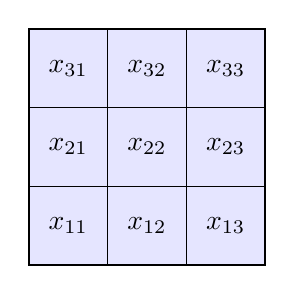
\begin{tikzpicture}[xscale=1,yscale=1]
\draw [fill=blue!10!white, thick] (0,0) rectangle (3, 3);
\draw (0,1) -- (3,1);
\draw (0,2) -- (3,2);
\draw (1,0) -- (1,3);
\draw (2,0) -- (2,3);
\node at (0.5,0.5) {$x_{11}$};
\node at (1.5,0.5) {$x_{12}$};
\node at (2.5,0.5) {$x_{13}$};
\node at (0.5,1.5) {$x_{21}$};
\node at (1.5,1.5) {$x_{22}$};
\node at (2.5,1.5) {$x_{23}$};
\node at (0.5,2.5) {$x_{31}$};
\node at (1.5,2.5) {$x_{32}$};
\node at (2.5,2.5) {$x_{33}$};
\end{tikzpicture}
\caption{Each variable $x_{ij}$ is in $\{1,-1\}$. There are $6$ constraint: across any row, the total parity should be $1$ (that is $x_{i1}x_{i2}x_{i3}=1$ for all $i\in \{1,2,3\}$) and across any column the total parity should be $-1$ (that is $x_{1i}x_{2i}x_{3i}=-1$ for all $i\in \{1,2,3\}$).}
\label{fig:magicsquare}
\end{figure}
The largest fraction of constraints satisfiable by assignments to (classical) variables $x_{ij}$ is 
\begin{enumerate}
\item $1$.
\item $\frac{5}{6}$.
\item $\frac{2}{3}$.
\item $\frac{1}{2}$.
\end{enumerate}

\noindent {\bf Answer: (b)}

\noindent {\bf Comments: }
We can easily find a case that satisfies 5 rows/columns, but satisfying all of them would require all the elements to multiply to both 1 and -1

\item {\bf Searching:} Consider a database of $N$ items, such that one unknown item is marked and the remaining items are unmarked. There is a randomized algorithm that can find the marked item with probability at least $\frac{1}{2}$ by looking at no more than $\rule{0.5cm}{0.05cm}$ items. However, any randomized algorithm that can find a marked item with probability at least $\frac{1}{2}$ must look at least at $\rule{0.5cm}{0.05cm}$ items.  
\begin{enumerate}
\item $N\ln 2$ and $N/2$.
\item $N$ and $1+N\ln 2$.
\item $\sqrt{N}$ and $\sqrt{\pi N/4}$.
\item $N/10$ and $N^{0.99}$.
\end{enumerate}

\noindent {\bf Answer: (a)}

\noindent {\bf Comments:}
Since there are $N$ elements and only one is marked, we must sample at least $N/2$ elements on average no matter how good our algorithm is.

\item {\bf Boosting:} A (randomized) algorithm $\cA$ takes as input a sample $r$ from a distribution $R$ and an input $x\in \cX$, to output $\cA(x,r)\in \{0,1\}$. It computes a given function $f:\cX\rightarrow \{0,1\}$ in the following sense: $\prob_{r\sim R}[\cA(x,r)=f(x)]\geq \frac{2}{3}$ for all $x\in \cX$. Let us say that $\frac{2}{3}$ is the \textit{success probability} of $\cA$. It is possible to boost this success probability to $1-\eps$ (for any $\eps\in (0,1)$), by running $\cA$ many times and taking the majority of the outputs. The number of times $\cA$ is run is best written as:     
\begin{enumerate}
\item $\omeg{\log\frac{1}{\eps}}$.
\item $\omeg{\sqrt{\log\frac{1}{\eps}}}$.
\item $\omeg{\log\log\frac{1}{\eps}}$.
\item This scheme will not work in general.
\end{enumerate}

\noindent {\bf Answer: (a)}

\noindent {\bf Comments:}
We can find this using the CLT on the sum of $A(x,r_i)$ for all samples $r_i$.

\item {\bf Boosting again:} Now, suppose the randomized algorithm $\cA$ computes a given function $f:\cX\rightarrow \{0,1\}$ in the following sense: $\prob_{x\sim U, r\sim R}[\cA(x,r)=f(x)]\geq \frac{2}{3}$, where $U$ is the uniform distribution over $\cX$. It is still possible to boost this success probability (now averaged according to $U$) to $1-\eps$, by running $\cA$ as many times as before and taking the majority of the outputs.     
\begin{enumerate}
\item I totally agree.
\item Yes, but it suffices to run $\cA$ way less times.
\item Yes, but in some cases $\cA$ needs to be run many more times.
\item This scheme will not work on some algorithms.
\end{enumerate}

\noindent {\bf Answer: (c)}

\noindent {\bf Comments:}
This is the same as 4 but we have to end up running it for each $x\in \mathcal{X}$, which takes a lot more time.

\item {\bf Correlation:} Given two $n$-bit strings $x,y$, our goal is to design a randomized algorithm $\cA$ that outputs a good estimate to $\frac{1}{n}\sum_i x_iy_i$ (the correlation between the strings). More precisely, given an error parameter $\eps$, the algorithm must output a real number $r(x,y)$ such that with probability at least $\frac{2}{3}$, $|r(x,y)-\frac{1}{n}\sum_i x_iy_i|\leq \eps$ (for all $x,y$). However, an unreasonable constraint is imposed upon the algorithm: it can only see one bit of the inputs $x,y$ at one time. Which of the following best captures the number of bits of input $\cA$ needs to see, as well as the tightest lower bound.
\begin{enumerate}
\item $\omeg{\log\frac{1}{\eps}}$. 
\item $\omeg{\frac{1}{\eps^2}}$.
\item $\omeg{2^{\frac{1}{\eps}}}$.
\item None of the above.
\end{enumerate}

\noindent {\bf Answer: (b)}

\noindent {\bf Comments:}
(a) grows too slow and (c) grows too fast.

\item {\bf Random walks:} A popular algorithmic framework is the random walk, which helps us sample from complicated distributions by taking some elementary steps. Given a connected and undirected graph $G=(V,E)$, a random walk inputs a distribution over $V$ and outputs another distribution over $V$. More precisely, it is a stochastic matrix $\{M_{x,y}\}_{x,y\in V}$ such that $M_{x,y}$ is non-zero iff $(x,y)\in E$ or $y=x$. The entry $M_{x,y}$ can be interpreted as the probability to reach $y$ starting from $x$. Note that there is some non-zero probability for self-transition on each $x$. Choose all the correct options:
\begin{enumerate}
\item Starting from any distribution, the random walk will converge to the uniform distribution over $V$.  
\item Starting from any distribution, the random walk will converge to a non-uniform distribution in which the vertices of higher degree have higher probability.
\item The rate of convergence to the stationary distribution is inversely related to the spectral gap\footnote{The difference between the absolute values of the largest eigenvalue and the second largest eigenvalue.} of the stochastic matrix $M$.
\item The rate of convergence to the stationary distribution is proportionally related to the spectral gap of the stochastic matrix $M$.
\end{enumerate}

\noindent {\bf Answer: (b), (d)}

\noindent {\bf Comments:}

The random walk will converge on a stationary state with higher probability in vertices with many edges with high weights, since more probability will move towards those points every step. Also, the spectral gap determines how fast eigenvector components of the state with eigenvalues less than 1 will decay, so a larger gap will lead to higher decay of those components and faster convergence.

\item {\bf Classical no-cloning:} Continuing the topic of stochastic processes, let's try to design certain stochastic matrix $M_{x,(y,z)}$, where $x\in \cX$ and $(y,z)\in \cX\times \cX$. The goal is to specify the entries of $M$ such that for any probability distribution $Q$ (viewed as a row matrix) over $\cX$, $Q\cdot M$ is equal to the distribution $Q\otimes Q$ over $\cX\times \cX$. Here, the notation $\otimes$ refers to the Kronecker product. Choose a correct option:  
\begin{enumerate}
\item It is possible to find such a stochastic matrix $M$.
\item Such a stochastic matrix can't exist since things should be linear.
\item Such a stochastic matrix can't exist since the total variational distance between two distributions $Q$ and $Q'$ is smaller than the total variational distance\footnote{Total variational distance measures how different two probability distributions are. Given two distributions $P_1, P_2$ over a set $\cX$, total variational distance is defined as $\frac{1}{2}\sum_{x\in \cX} |P_1(x)-P_2(x)|$.} between $Q\times Q$ and $Q'\times Q'$.
\item Such a stochastic matrix can't exist, but for very different reasons not listed above.
\end{enumerate}

\noindent {\bf Answer: (b)}

\noindent {\bf Comments:}
This operation isn't linear because $(Q+Q')\cdot M\neq Q\otimes Q+Q'\otimes Q'$.

\item {\bf Matrices:} Selection all correct statements about matrices (with entries as complex numbers):
\begin{enumerate}
\item A square matrix $M$ is diagonalizable if there is another square matrix $N$ and a diagonal matrix $D$ such that $M=N D N^{-1}$.
\item Every square matrix has singular-value decomposition, however not every square matrix has an eigen-value decomposition. 
\item A unitary matrix may not be hermitian, hence it may not have eigenvalues.
\item Singular values of a square matrix are always non-negative reals, but eigenvalues of a hermitian matrix may be complex numbers.
\end{enumerate}

\noindent {\bf Answer: (a), (b)}

\noindent {\bf Comments:}
\end{enumerate}


\end{document}
